\documentclass[10pt,preprint]{aastex}
\usepackage{psboxit}

\newcommand{\kms}{\,km~s$^{-1}$}
\def\squig{\sim\!\!}
\newcommand{\Msun}{\mbox{\,$M_{\odot}$}}
\newcommand{\Lsun}{\mbox{\,$L_{\odot}$}}

\PScommands
\newcommand{\graybox}[1]{\psboxit{box 0.7 setgray fill}{\spbox{#1}}}

\newcommand{\mdmlimit}{0.5}
\newcommand{\vmaxmean}{56}
\newcommand{\mrmean}{-14.7}

\newcommand{\latin}[1]{{#1}}
\newcommand{\ie}{\latin{i.e.}}
\newcommand{\eg}{\latin{e.g.}}
\newcommand{\cf}{\latin{c.f.}}
\newcommand{\Sersic}{S\'ersic}
\newcommand{\vv}[1]{{\bf #1}}
\newcommand{\df}{\delta}
\newcommand{\dfft}{{\tilde{\delta}}}
\newcommand{\betaft}{{\tilde{\beta}}}
\newcommand{\erf}{{\mathrm{erf}}}
\newcommand{\erfc}{{\mathrm{erfc}}}
\newcommand{\Step}{{\mathrm{Step}}}
\newcommand{\ee}[1]{\times 10^{#1}}
\newcommand{\avg}[1]{{\langle{#1}\rangle}}
\newcommand{\Avg}[1]{{\left\langle{#1}\right\rangle}}
\def\simless{\mathbin{\lower 3pt\hbox
    {$\,\rlap{\raise 5pt\hbox{$\char'074$}}\mathchar"7218\,$}}} % < or of order
\def\simgreat{\mathbin{\lower 3pt\hbox
    {$\,\rlap{\raise 5pt\hbox{$\char'076$}}\mathchar"7218\,$}}} % > or of order
\newcommand{\iras}{{\sl IRAS\/}}
\newcommand{\petroratio}{{{\mathcal{R}}_P}}
\newcommand{\petroradius}{{{r}_P}}
\newcommand{\petronumber}{{{N}_P}}
\newcommand{\petroratiolim}{{{\mathcal{R}}_{P,\mathrm{lim}}}}
\newcommand{\band}[2]{\ensuremath{^{#1}\!{#2}}}
\newcommand{\Vmax}{\ensuremath{V_\mmax}}
\newcommand{\mmax}{\ensuremath{\mathrm{max}}}
\newcommand{\mmin}{\ensuremath{\mathrm{min}}}
\newcommand{\minmax}{\ensuremath{\mathrm{\left\{^{min}_{max}\right\}}}}
\newcommand{\fixMr}{\ensuremath{M_\fixr}}
\newcommand{\fixr}{\ensuremath{{r}}}
\newcommand{\fixredshift}{0.1}
\newcommand{\fixmag}[1]{\ensuremath{{^{\fixredshift}\!{#1}}}}

\setlength{\footnotesep}{9.6pt}

\newcounter{thefigs}
\newcommand{\fignum}{\arabic{thefigs}}

\newcounter{thetabs}
\newcommand{\tabnum}{\arabic{thetabs}}

\newcounter{address}

\shortauthors{Blanton {\it et al.} (2006)}
\shorttitle{Notes on NSA tests with Simard Catalog}

\begin{document}

\title{Notes on Tests of NASA-Sloan Atlas Fluxes:\\
Tests against Simard GIM2D Models and Measurements}


\author{
Michael R. Blanton\altaffilmark{\ref{NYU}}
}

%\altaffiltext{1}{Based on observations obtained with the
%Sloan Digital Sky Survey\label{SDSS}}
\setcounter{address}{1}
\altaffiltext{\theaddress}{
    \stepcounter{address}
    Center for Cosmology and Particle Physics, Department of Physics, New
    York University, 4 Washington Place, New
    York, NY 10003
    \label{NYU}}

\begin{abstract}
I test the NASA-Sloan Atlas measurements of flux and sizes against
those of \citet{simard11a}, concentrating on galaxies brighter than
$r\sim16.5$. First, for galaxies from the \citet{simard11a} catalog, I
create a set of 5000 simulated images, to which I apply the NSA flux
and size measurement procedure. From these measurements I demonstrate
that for these models Petrosian quantities defined with elliptical
apertures, including the flux and $r_{50}$ values, agree well with the
intrinsic properties of the models.  {\bf Should I try to find pure
Petro quantity?}.  The trends in the measured quantities as a function
of size seem to be due to intrinsic correlations between angular size
and the galaxy profile properties {\bf test this}. Circularized
Petrosian quantities have several biases that affect them, as do
single-component \Sersic\ model fits. Second, we match the
\citet{simard11a} catalog to the NSA catalog and test the differences
between the analysis techniques for real data. The differences reflect
the differences seen for the model data.
\end{abstract}

\setcounter{thefigs}{0}

\section{Code, Data, and Methods} 
\label{sec:code}

These tests were done using the {\tt dimage} software used for the
NASA-Sloan Atlas processing, described in \citet{blanton11a}. This was
around revision {\tt r1116} of that code. 

The \citet{simard11a} catalog I used was the pure de Vaucouleurs plus
exponential fit, as downloaded as a FITS file from Vizier. Where
necessary, I matched this to the NSA with a 2 arcsec tolerance. I
trimmed the \citet{simard11a} catalog for the plots to only include
galaxies with $r_{50}>2$ pixels, which eliminated 5-10\% of the
objects; 99\% of the objects smaller than that were stars on visual
inspection.

The NSA data was from {\tt v1\_0\_0}, which was the revision to include
galaxies up to $z=0.15$. The code reanalyzed the child images for the
$r$-band from that data. The NSA already includes circularized
Petrosian quantities as well as single-component \Sersic\ fits. This
data resides on riemann at:
\begin{center}
{\tt /clusterfs/riemann/raid000/blanton/atlas} 
\end{center}
This is referred to below as {\tt \$ATLAS\_DATA}. The {\tt v1\_0\_0}
catalog is in the {\tt v1} subdirectory. This is accessible on the
SDSS-III site:
\begin{center}
{\tt http://data.sdss3.org/sas/ebosswork/manga/atlas}
\end{center}

The Petrosian method tested uses an estimate of an axis ratio $b/a$
(minor over major) and position angle $\phi$ to define a set of
elliptical annuli. Otherwise it uses the standard algorithm for
Petrosian magnitudes, with the Petrosian radius $R_P$ defined as the
semimajor axis of the ellipse where the Petrosian ratio $\eta= I/\bar
I = 0.2$, and with the aperture for the flux defined with a radius
$2R_P$. I measure $R_{50}$ and $R_{90}$ as the ellipses whose the
semimajor axes enclose 50\% and 90\% of the flux within $2R_P$. Within
about 2 pixels the method is approximate; in practice, the Petrosian
radius as usually defined has a radius of 4--5 pixels in SDSS data, so
this is adequate for our purposes here.

Several choices are available for defining $b/a$ and $\phi$. The NSA
determines axis ratios based on second moments within its
(circularized) Petrosian $R_{50}$ and $R_{90}$, as well based on its
single-component \Sersic\ fit. 

In detail, the elliptical Petrosian measurement is done with a piece
of python code ({\tt petro.py}) called by an executable script {\tt
petro2d}. The outputs are put into each atlas image directory next to
the measurement files. The calculation takes somewhat less than 1
second per image on average.

\section{Tests against models} 
\label{sec:models}

To test the code and investigate the reliability of this method in a
controlled environment, I put together a set of 10,000 simulated
images (code used was {\tt simard_tests.pro}). These images were based
\citet{simard11a} catalog parameters for a randomly selected set of
objects with $r<16.5$, roughly the limit for MaNGA. I created fake
images with roughly the sky noise of SDSS data (around 0.03 nmgy per
pixel in the $r$-band) and with typical-to-good SDSS seeing (a FWHM of
2.84 pixels, or 1.1 arcsec). In detail, the seeing was modeled as a
set of three axisymmetric concentric Gaussians). \citet{simard11a}
provides a model-based definition of half-light ratio, which is to
project each model component onto its major axis (which can differ),
sum the result, and calculate the half-light radius on that sum. {\bf
	check that this is exactly what he did}

I ran the standard NSA measurement code on each fake galaxy (not
including the \Sersic\ fitting), and then the elliptical Petrosian
measurements. 

\stepcounter{thefigs}
\begin{figure}
\figurenum{\fignum}
\includegraphics[width=0.49\textwidth]{test-simard-petro-flux.ps} \quad
\includegraphics[width=0.49\textwidth]{test-simard-petro-r50.ps} 
\caption{\label{fig:rawrun} Data that our sky model is fit to, for
part of an SDSS drift scan run.  The vertical direction is the scan
direction ($y$), the horizontal direction is perpendicular to the scan
direction ($x$). This image is the 8$\times$8 binned flat-fielded SDSS
data. Areas where no objects were detected show the original data.
Areas where objects were detected are replaced by the background sky
estimate plus noise. Each of the six vertical stripes represents a
``camcol'' and the black areas in between are not covered by a
CCD. The units of the image are raw counts, which therefore reflect
the relative gains of the different CCDs. }
\end{figure}

\bibliographystyle{apj}
\bibliography{../../ccpp-latex/ccpp}

\end{document}
